\section{Electronics and Data Acquisition}
\label{secDAQ}

%\begin{floatingfigure}[l]{0.3\textwidth}
\begin{figure}[!t]
\centering
%\subfigure[]{
%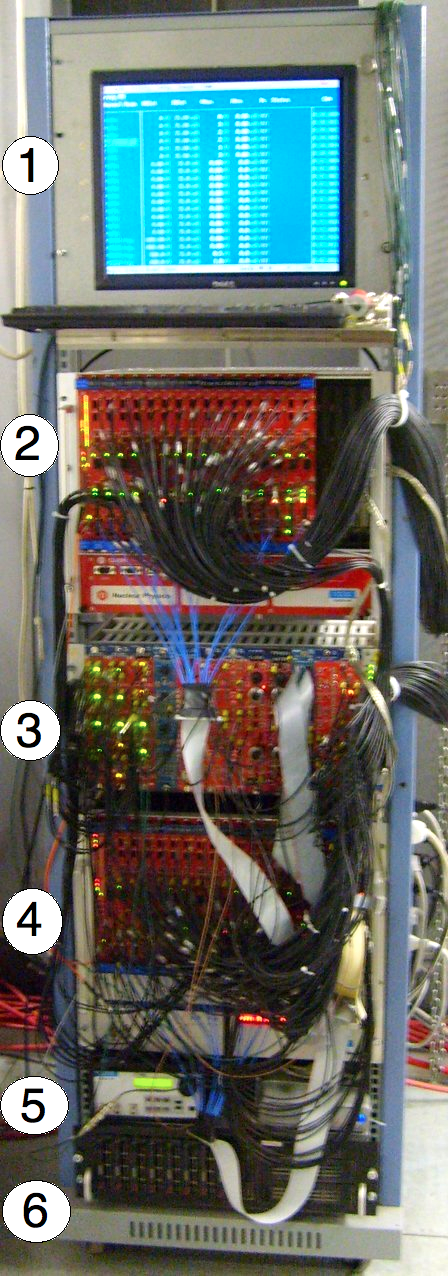
\includegraphics[height=0.5\linewidth]{plots/Detector/DAQ_withLabels.png}
%\label{figDAQ_1}}
%\subfigure[]{
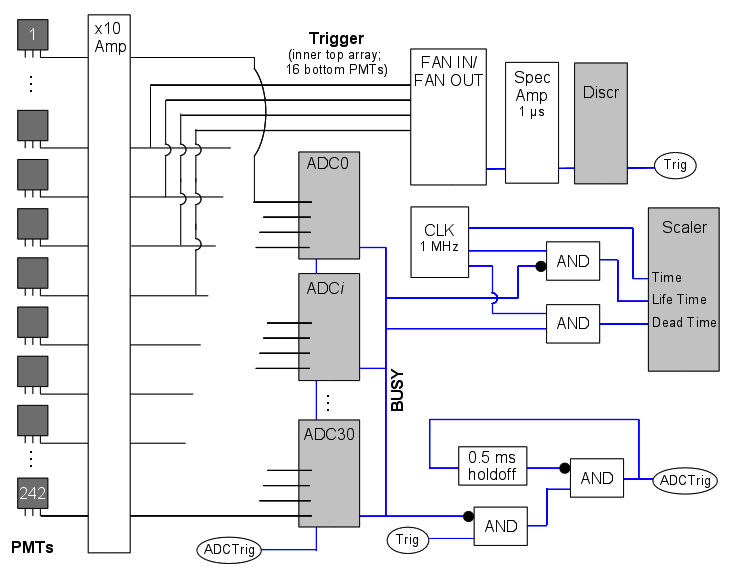
\includegraphics[width=0.9\linewidth]{plots/Detector/DAQschemeNew2.png}
%\label{figDAQ_2}}
%\caption[Schematics of the XENON100 data acquisition system]{SChematics of the XENON100 data acquisition system in the electronics rack: 1 - HV control panel; 2 and 4 - ADCs; 3 - clocks, FANs, discriminators, shaping amplifiers, gate generators,  scalers; 5 - LED pulser; 6 - storage disk. A scheme in Fig.~\ref{figDAQ_2} from Ref.~\cite{xe100-instrument}.}
\caption[Schematics of the XENON100 data acquisition system]{Schematics of the XENON100 data acquisition system. Figure from Ref.~\cite{xe100-instrument}.}
\label{figDAQ}
\end{figure}
%\end{floatingfigure}

\begin{figure}[!t]
\centering
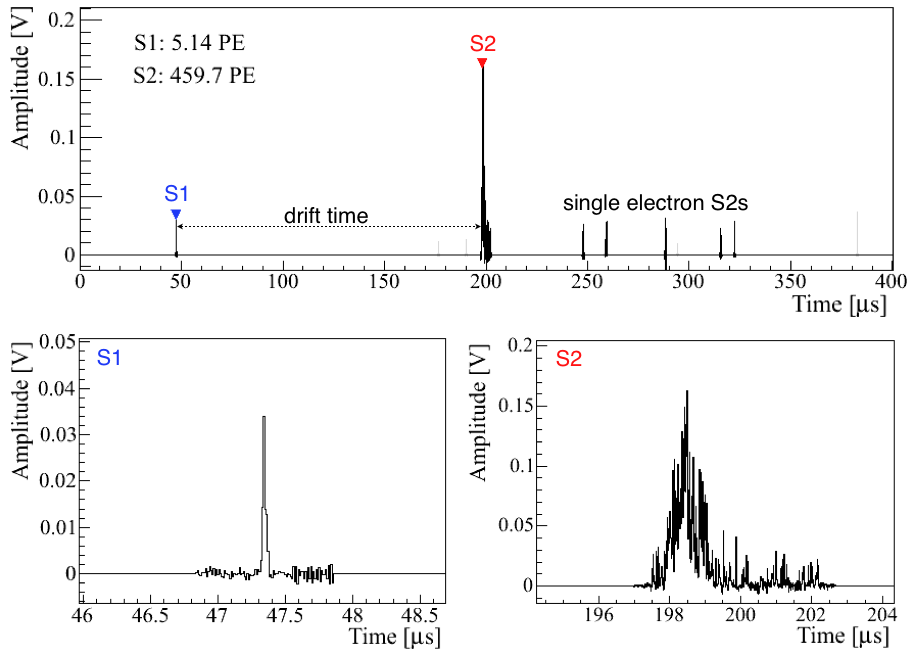
\includegraphics[width=0.9\linewidth]{plots/Detector/Waveform_withLabels.png}
\caption[A waveform of a low energy event in XENON100]{A waveform of a low energy event in XENON100. The bottom plots show a zoom into S1 and S2 peaks identified in the trace. The structures with the size of $<$40~PE after the main S2 peak are S2 signals from single electrons extracted into gas phase. Figure published in Ref.~\cite{xe100-instrument}.}
\label{figWaveform}
\end{figure}

The PMT signals are amplified by a factor 10 with Phillips PS776 amplifiers, and digitized with CAEN V1724 flash ADCs with 100~MHz sampling rate, 14~bit resolution, and 40~MHz bandwidth. The schematics of the XENON100 data acquisition system (DAQ) is shown in Fig.~\ref{figDAQ}. %The amplifiers are installed in NIM rack mounted on the shield door, and the other modules, together with high voltage control panel, in another electronics rack placed near the detector shield.

The DAQ digitizes the full waveform of the 242 PMTs, where the time window for an event is 400~$\mu$s, more than twice the maximum electron drift time (see Fig.~\ref{figWaveform}) of 176~$\mu$s at the drift field of 0.53~kV/cm. This allows to not miss any waveform information, regardless wether the trigger is generated by S1 or S2 signal.  
Using circular buffers in flash ADCs, with 512~kB memory per channel, the DAQ samples continuously, and stores the data if a trigger occurs. The data is stored in zero length encoding (ZLE) mode: only samples that exceed a certain threshold are stored, together with some samples before and after the threshold crossing. The ZLE threshold is defined by the size of the noise pulses on a given channel, and for 98\% of the PMTs is set to 30~ADC counts (4~mV), which corresponds to $\sim$0.3~photoelectrons (PE). For some noisy channels it is at higher values:  45~ADC counts for a few bottom PMTs, and 100~ADC counts for top PMTs 1 and 2.

Trigger system can be based on S1 or S2 signals. The latter provides a significantly lower energy threshold. 
The analog signal of the inner 64 top array PMTs and the 16 channels in the bottom array is summed using linear FANs, and used in the S2 trigger. The fraction of full S2 signal seen by the PMTs used for the trigger is 52\%, which results in a threshold of $\sim$300~PE. Before the summed signal is fed into a low energy discriminator, it is integrated with a time constant of 1~$\mu$s and shaped with a spectroscopy amplifier. 
In case no potential is applied to the cathode, the electrons are not drifted to the gas phase, and proportional scintillation signal (S2) is not generated. For the S1 trigger, the majority signal of the ADCs is used, which is 125~mV for every channel that shows a signal above the threshold, which is set to 0.5~PE.  Due to short time coincidence of the majority signal (10~ns) the threshold in this configuration is higher. 
A trigger hold-off with time window 500~$\mu$s, which is done with a NIM gate generator, disables a new event following immediately after the current one.

In order to reduce the count rate in those calibration runs, where only the low energy region is relevant for dark matter search, the high energy (HE) veto is implemented to remove the high energetic signals from the data set, which inhibits events triggered by the S1 signal. The peaks with narrow width are selected by shaping and differentiating the signal with a spectroscopy amplifier.

The measurements and data storage are performed with the XENON Data Acqusition software program (DAX). The settings for the data acquisition are defined in {\it xml}-files. For each acquired data set, it generates an ASCII log file that contains information about the measurement (file name, timing, settings) and scaler values. DAX can be also run in oscilloscope mode, which provides real time access to the digitized waveforms.

The data is stored in the general-purpose XENON Data Input Output (XDIO) file format with an indexed file header, which allows to jump directly to a specific event or a PMT in order to speed up the analysis.

The raw data is converted to physical parameters using the XENON Raw Data Processor (XERAWDP), a ROOT~\cite{ROOT} based C++ program specifically developed for the XENON100 data analysis, but with a design that should allow processing of raw data from other liquid xenon detectors due to highly configurable modules, generic module interfaces, and parameters specified with $xml$ configuration files.

The data conversion proceeds in three broad stages: pre-processing the waveforms, searching for peak candidates, and computing the reduced quantities associated with each of them.
In the pre-processing stage, the baseline of each ZLE block of each waveform included in the event is computed on 46 samples, and the waveforms are converted from ADC counts to volts~(Fig.~\ref{figWaveform}). The waveforms of all target volume channels are added into a total waveform that is used to search for S1 and S2 peak candidates, and the waveforms of the veto volume channels are also added into a total veto waveform that is used to search for S1 peak candidates. The peak finding in the target volume waveform is done in two steps. First, XERAWDP searches for S2-like peaks in the entire summed waveform, and then looks for S1-like peaks in between all S2 peak candidates. In order to facilitate the detection of the extent of S2 peaks, 
the S2 peak finding algorithm starts by applying a digital filter to the entire waveform and smoothing out the high frequency components. The algorithm does not search for S2 peaks after the first S2 peak which exceeds the threshold, in order to avoid mis-identification of the signals due to after-pulsing and single electron S2s. 

%The Xenon Raw Data Processor (xerawdp) program creates root files with �physical� quantities from the raw data (.xed) files with the 242 PMT digitized traces. It is used to convert all source data taken with the detector except LED calibration data. The main steps are
%     Read raw data for an event
%      Compute baselines, sum all relevant channels into summed waveforms
%      Identify S1 like peaks and/or S2 like peaks in the summed waveforms
%      Compute a multitude of parameters for each peak candidate
%      Compute the S2 xy positions using all available position reconstruction algorithms
%      Apply position dependent corrections


%It then searches the filtered waveform for regions where the signal exceeds a threshold of 10~mV  for at least 0.6~$\mu$s, a time interval large enough to contain at least one S2 peak, and for which the preceding and following 0.21~us have an average signal less than 5\% of the maximum within the interval.

%The interval above the threshold often contains multiple peaks due to the long after-pulsing tails that follow large S2 peaks.

%The algorithm then recursively searches for S2-like peaks within that interval. This is done by computing the extent of any potential peak by starting from its maximum sample in the interval and going backward in the trace until either the signal drops below 0.5\% (s2/large_peaks/left_height_fraction_threshold) of its maximum or the slope of the signal changes sign. This defines the left boundary of this peak. The same procedure is repeated going forward in the trace to find the right boundary. If the peak found has a FWHM larger than 0.35 us (s2/large_peaks/min_width) � much smaller than typical S2 widths observed, see for example s2width � it will be considered as a valid S2 peak candidate and its location and boundaries will be saved. The recursive search for S2 peaks then continues within the interval (excluding the regions where any peaks might already have been found). This first part of the algorithm will detect S2-like peaks down to very low energies (~150 pe) with close to 100% efficiency.

%After searching for large S2 peak candidates the S2 peak finding algorithm proceeds to search for the smallest of S2 peaks from tens all the way down to one electron (~17 pe) S2 peaks. A digital filter (s2/tiny_peaks/filter) with a higher frequency cut-off is applied to the waveform to identify regions where its average height exceeds what is expected for a single electron S2 signal, roughly tens of photoelectrons over 0.5 us (can be computed knowing the proportional gap, electric field, electroluminesce yield, etc). Any interval on the filtered waveform exceeding 1 mV (s2/tiny_peaks/signal_threshold) for more than 0.4 us (s2/tiny_peaks/min_interval_width) for which the preceding and following 0.1 us (s2/tiny_peaks/pre,post_peak_avg_window) have an average signal less than 5% of the maximum of the interval and with an interval maximum over interval width ratio larger than 1 mV/sample (s2/tiny_peaks/aspect_ratio_threshold) will be considered as an S2 peak candidate. All S2 peaks found are sorted in decreasing order of size (in mV*ns) and the positions and boundaries of the 32 (s2/max_nb_peaks) largest S2 peak candidates are kept.

%The S1 peak finding algorithm searches the total waveform for signal excursions of at least 3 mV (s1/signal_threshold) above the baseline. The boundaries of the peak candidate are defined as the points where the signal drops below 0.5% (s1/height_fraction_threshold) of its maximum, for more than 20 ns (s1samples_below_threshold). If all of the following conditions are met the location and boundaries of the S1 peak peak candidate will be kept: the 0.5 us (s1/pre_peak_avg_window/) preceding the peak and the 100 ns (s1/post_peak_avg_window) following the peak respectively have an average signal less than 1% (s1/pre_peak_avg_threshold) and 4% (s1/post_peak_avg_threshold) of the maximum; the FWHM of the filtered (s1/filter) trace near the peak candidate is smaller than 0.5 us (s1/filtered_width_threshold), to distinguish them from single electron S2s; the maximum is at least 3 times larger (s1/negative_excursion_fraction_threshold) than the largest negative excursion in the vicinity of the peak. The parameters of the 32 (s1/max_nb_peaks) largest S1 peaks identified are kept. 

%A peak is required to pass a 50~mV threshold, in order to be recognized as an S2.
%A 50~mV threshold is required S2 peaks, in order to avoid selecting as S1 candidates 
%This condition is used since we expect the S1 signal to preceed any S2 signal and to avoid selecting as S1 peak candidates the many photoelectrons that typically follow a large S2 peak (PMT afterpulses, single electron S2s, etc). 


